%  LaTeX support: latex@mdpi.com 
%  In case you need support, please attach all files that are necessary for compiling as well as the log file, and specify the details of your LaTeX setup (which operating system and LaTeX version / tools you are using).

% You need to save the "mdpi.cls" and "mdpi.bst" files into the same folder as this template file.

%=================================================================
\documentclass[jof,article,submit,moreauthors,pdftex,10pt,a4paper]{Definitions/mdpi} 

% If you would like to post an early version of this manuscript as a preprint, you may use preprint as the journal and change 'submit' to 'accept'. The document class line would be, e.g., \documentclass[preprints,article,accept,moreauthors,pdftex,10pt,a4paper]{mdpi}. This is especially recommended for submission to arXiv, where line numbers should be removed before posting. For preprints.org, the editorial staff will make this change immediately prior to posting.

%
%--------------------
% Class Options:
%--------------------
% jof
%----------
% Choose between the following MDPI journals:
% acoustics, actuators, addictions, admsci, aerospace, agriculture, agronomy, algorithms, animals, antibiotics, antibodies, antioxidants, applsci, arts, asi, atmosphere, atoms, axioms, batteries, bdcc, behavsci, beverages, bioengineering, biology, biomedicines, biomimetics, biomolecules, biosensors, brainsci, buildings, carbon, cancers, catalysts, cells, ceramics, challenges, chemengineering, chemosensors, children, cleantechnol, climate, clockssleep, cmd, coatings, colloids, computation, computers, condensedmatter, cosmetics, cryptography, crystals, cybersecurity, data, dentistry, designs, diagnostics, dairy, diseases, diversity, drones, econometrics, economies, education, electrochem, electrochemistry, electronics, energies, entropy, environments, epigenomes, est, fermentation, fibers, fire, fishes, fluids, foods, forecasting, forests, fractalfract, futureinternet, galaxies, games, gastrointestdisord, gels, genealogy, genes, geohazards, geosciences, geriatrics, hazardousmatters, healthcare, heritage, highthroughput, horticulturae, humanities, hydrology, informatics, information, infrastructures, inorganics, insects, instruments, ijerph, ijfs, ijms, ijgi, ijtpp, inventions, j, jcdd, jcm, jcs, jdb, jfb, jfmk, jimaging, jof, jintelligence, jlpea, jmmp, jmse, jpm, jrfm, jsan, land, languages, laws, life, literature, logistics, lubricants, machines, magnetochemistry, make, marinedrugs, materials, mathematics, mca, medsci, medicina, medicines, membranes, metabolites, metals, microarrays, micromachines, microorganisms, minerals, modelling, molbank, molecules, mps, mti, nanomaterials, ncrna, neonatalscreening, neuroglia, nitrogen, nutrients, ohbm, particles, pathogens, pharmaceuticals, pharmaceutics, pharmacy, philosophies, photonics, plants, plasma, polymers, polysaccharides, proceedings, processes, proteomes, publications, quaternary, qubs, reactions, recycling, religions, remotesensing, reports, resources, risks, robotics, safety, sci, scipharm, sensors, separations, sexes, sinusitis, smartcities, socsci, societies, soilsystems, sports, standards, stats, surfaces, surgeries, sustainability, symmetry, systems, technologies, toxics, toxins, tropicalmed, universe, urbansci, vaccines, vehicles, vetsci, vibration, viruses, vision, water, wem, wevj
%---------
% article
%---------
% The default type of manuscript is article, but can be replaced by: 
% abstract, addendum, article, benchmark, book, bookreview, briefreport, casereport, changes, comment, commentary, communication, conceptpaper, correction, conferenceproceedings, conferencereport, expressionofconcern, extendedabstract, meetingreport, creative, datadescriptor, discussion, editorial, essay, erratum, hypothesis, interestingimages, letter, meetingreport, newbookreceived, opinion, obituary, projectreport, reply, reprint, retraction, review, perspective, protocol, shortnote, supfile, technicalnote, viewpoint
% supfile = supplementary materials
% protocol: If you are preparing a "Protocol" paper, please refer to http://www.mdpi.com/journal/mps/instructions for details on its expected structure and content.
%----------
% submit
%----------
% The class option "submit" will be changed to "accept" by the Editorial Office when the paper is accepted. This will only make changes to the frontpage (e.g., the logo of the journal will get visible), the headings, and the copyright information. Also, line numbering will be removed. Journal info and pagination for accepted papers will also be assigned by the Editorial Office.
%------------------
% moreauthors
%------------------
% If there is only one author the class option oneauthor should be used. Otherwise use the class option moreauthors.
%---------
% pdftex
%---------
% The option pdftex is for use with pdfLaTeX. If eps figures are used, remove the option pdftex and use LaTeX and dvi2pdf.

%\usepackage{biblatex}
\usepackage{xcolor}
%\addbibresource{mendeley_v2.bib}
\newcommand{\textlower}{$<$}
\newcommand{\TODO}[1]{\textbf{\color{red}{#1}}}
\newcommand{\exoDer}{\textit{Exophiala dermatitidis}}
\newcommand{\exoMes}{\textit{Exophiala mesophila}}
\newcommand{\exoSid}{\textit{Exophiala sideris}}
\newcommand{\exoSpi}{\textit{Exophiala spinifera}}
\newcommand{\claImm}{\textit{Cladophialophora immunda}}
\newcommand{\fonPed}{\textit{Fonsacaea pedrosi}}
\newcommand{\horWer}{\textit{Hortaea werneckii}}
\newcommand{\canAlb}{\textit{Candida albicans}}
\newcommand{\aspNig}{\textit{Aspergillus niger}}
\newcommand{\aspNid}{\textit{Aspergillus nidulans}}
\newcommand{\aspFum}{\textit{Aspergillus fumigatus}}
\newcommand{\aspRub}{\textit{Aspergillus ruber}}
\newcommand{\penChr}{\textit{Penicillium chrysogenum}}
\newcommand{\debFab}{\textit{Debaryomyces fabryi}}
\newcommand{\debHan}{\textit{Debaryomyces hansenii}}
\newcommand{\walIch}{\textit{Wallemia ichthyophaga}}
\newcommand{\walMel}{\textit{Wallemia mellicola}}
\newcommand{\canPar}{\textit{Candida parapsilosis}}
\newcommand{\cocImm}{\textit{Coccidioides immitis}}
\newcommand{\triRub}{\textit{Trichophyton rubrum}}
\newcommand{\thiTer}{\textit{Thielavia terrestris}}
\newcommand{\mycThe}{\textit{Myceliophthora thermophila}}
\newcommand{\neuCra}{\textit{Neurospora crassa}}
\newcommand{\sacCer}{\textit{Saccharomyces cerevisiae}}
\newcommand{\schPom}{\textit{Schizosaccharomyces pombe}}
\newcommand{\cryNeo}{\textit{Cryptococcus neoformans}}
\newcommand{\micCan}{\textit{Microsporum canis}}
\newcommand{\onyCor}{\textit{Onygena corvina}}
\newcommand{\blaDer}{\textit{Blastomyces dermatitidis}}
\newcommand{\parBra}{\textit{Paracoccidioides brasiliensis}}
\newcommand{\cocPos}{\textit{Coccidioides posadasii}}
\newcommand{\toxGon}{\textit{Toxoplasma gondii}}
\newcommand{\fusOxy}{\textit{Fusarium oxysporum}}
\newcommand{\fusSol}{\textit{Fusarium solani}}
\newcommand{\tryRub}{\textit{Fusarium solani}}
\newcommand{\clado}{\textit{Cladophialophora}}
\newcommand{\attspe}{\textit{Attalea speciosa}}
\newcommand{\claban}{\textit{Cladophialophora bantiana}}
\newcommand{\clasat}{\textit{Cladophialophora saturnica}}
\newcommand{\clapsa}{\textit{Cladophialophora psammophila}}
\newcommand{\clasph}{\textit{Cladosporium sphaerospermum}}
\newcommand{\claBan}{\textit{Cladophialophora bantiana}}
\newcommand{\fusGra}{\textit{Fusarium graminearum}}
\newcommand{\fusSpo}{\textit{Fusarium sporotrichoides}}
\newcommand{\triAru}{\textit{Trichoderma arundinaceum}}
\newcommand{\triBre}{\textit{Trichoderma brevicompactum}}
\newcommand{\phiSp}{\textit{Aspergillus salisburgensis}}
\newcommand{\phiScl}{\textit{Aspergillus sclerotialis}}
\newcommand{\staCha}{\textit{Stachybotrys chartarum}}
\newcommand{\staChl}{\textit{Stachybotrys chloronata}}
\newcommand{\ustMay}{\textit{Ustilago maydis}}
\newcommand{\exo}{\textit{Exophiala}}
\newcommand{\herpo}{\textit{Herpotrichiellaceae}}
\newcommand{\skin}{skin}
\newcommand{\tol}{\textit{toluene}}
\newcommand{\glu}{\textit{glucose}}

%=================================================================
\firstpage{1} 
\makeatletter 
\setcounter{page}{\@firstpage} 
\makeatother
\pubvolume{xx}
\issuenum{1}
\articlenumber{5}
\pubyear{2018}
\copyrightyear{2018}
%\externaleditor{Academic Editor: name}
\history{Received: date; Accepted: date; Published: date}
%\updates{yes} % If there is an update available, un-comment this line

%% MDPI internal command: uncomment if new journal that already uses continuous page numbers 
%\continuouspages{yes}

%------------------------------------------------------------------
% The following line should be uncommented if the LaTeX file is uploaded to arXiv.org
%\pdfoutput=1

%=================================================================
% Add packages and commands here. The following packages are loaded in our class file: fontenc, calc, indentfirst, fancyhdr, graphicx, lastpage, ifthen, lineno, float, amsmath, setspace, enumitem, mathpazo, booktabs, titlesec, etoolbox, amsthm, hyphenat, natbib, hyperref, footmisc, geometry, caption, url, mdframed, tabto, soul, multirow, microtype, tikz

%=================================================================
%% Please use the following mathematics environments: Theorem, Lemma, Corollary, Proposition, Characterization, Property, Problem, Example, ExamplesandDefinitions, Hypothesis, Remark, Definition
%% For proofs, please use the proof environment (the amsthm package is loaded by the MDPI class).

%=================================================================
% Full title of the paper (Capitalized)
\Title{Back to the salt mines: genome and transcriptome comparisons of the halophilic fungus Aspergillus salisburgensis and its halotolerant relative Aspergillus sclerotialis }

% Author Orchid ID: enter ID or remove command
%\newcommand{\orcidauthorA}{0000-0000-000-000X} % Add \orcidA{} behind the author's name
%\newcommand{\orcidauthorB}{0000-0000-000-000X} % Add \orcidB{} behind the author's name

% Authors, for the paper (add full first names)
\Author{Hakim Tafer $^{1,*}$, Caroline Poyntner $^{1}$, Ksenija Lopandic $^{1}$, Katja Sterflinger $^{1}$ and Guadalupe Pi\~nar $^{1}$}

% Authors, for metadata in PDF
\AuthorNames{Hakim Tafer , Caroline Poyntner , Ksenija Lopandic and Guadalupe Pi\~nar}

% Affiliations / Addresses (Add [1] after \address if there is only one affiliation.)
\address{%
$^{1}$ \quad Extremophiles Center, Department of Biotechnology, University of Natural Resources and Life Sciences Muthgasse 18, 1190 Vienna, Austria\\
% Contact information of the corresponding author
\corres{Correspondence: hakim.tafer@boku.ac.at}}

% Current address and/or shared authorship
%\firstnote{Current address: Affiliation 3} 
%\secondnote{These authors contributed equally to this work.}
% The commands \thirdnote{} till \eighthnote{} are available for further notes

%\simplesumm{} % Simple summary

%\conference{} % An extended version of a conference paper

% Abstract (Do not insert blank lines, i.e. \\) 
\abstract{Salt mines are among the most extreme environments as they combine darkness, low nutrient availability and hypersaline conditions. Based on comparative genomics and transcriptomics, we describe in this work the adaptive strategies of the true halophile fungus {\phiSp} found in a salt mine in Austria and compare this strain to the ex-type halotolerant fungal strain {\phiScl}. On a genomic level, {\phiSp} exhibits a reduced genome size compared to {\phiScl} as well as a contraction of genes involved in transport processes. The proteome of {\phiScl} exhibits an increased proportion of alanine, glycine and proline compared to the proteome of non-halophilic species. Transcriptome analyses of both strains growing at 5$\%$ and 20$\%$ NaCl show that {\phiSp} regulates three times fewer genes than {\phiScl} in order to adapt to the higher salt concentration. In {\phiScl}, the increased osmotic stress impacted processes related to translation, transcription, transport and energy. In contrast, membrane-related and lignolytic proteins were significantly affected in {\phiSp}.}

% Keywords
\keyword{Halophiles; Halotolerant; fungi; transcriptomics; genomics; (list three to ten pertinent keywords specific to the article, yet reasonably common within the subject discipline.)}

% The fields PACS, MSC, and JEL may be left empty or commented out if not applicable
%\PACS{J0101}
%\MSC{}
%\JEL{}

%%%%%%%%%%%%%%%%%%%%%%%%%%%%%%%%%%%%%%%%%%
% Only for the journal Diversity
%\LSID{\url{http://}}

%%%%%%%%%%%%%%%%%%%%%%%%%%%%%%%%%%%%%%%%%%
% Only for the journal Applied Sciences:
%\featuredapplication{Authors are encouraged to provide a concise description of the specific application or a potential application of the work. This section is not mandatory.}
%%%%%%%%%%%%%%%%%%%%%%%%%%%%%%%%%%%%%%%%%%

%%%%%%%%%%%%%%%%%%%%%%%%%%%%%%%%%%%%%%%%%%
% Only for the journal Data:
%\dataset{DOI number or link to the deposited data set in cases where the data set is published or set to be published separately. If the data set is submitted and will be published as a supplement to this paper in the journal Data, this field will be filled by the editors of the journal. In this case, please make sure to submit the data set as a supplement when entering your manuscript into our manuscript editorial system.}

%\datasetlicense{license under which the data set is made available (CC0, CC-BY, CC-BY-SA, CC-BY-NC, etc.)}

%%%%%%%%%%%%%%%%%%%%%%%%%%%%%%%%%%%%%%%%%%
% Only for the journal Toxins
%\keycontribution{The breakthroughs or highlights of the manuscript. Authors can write one or two sentences to describe the most important part of the paper.}

%\setcounter{secnumdepth}{4}
%%%%%%%%%%%%%%%%%%%%%%%%%%%%%%%%%%%%%%%%%%
\begin{document}
%%%%%%%%%%%%%%%%%%%%%%%%%%%%%%%%%%%%%%%%%%
%% Only for the journal Gels: Please place the Experimental Section after the Conclusions

%%%%%%%%%%%%%%%%%%%%%%%%%%%%%%%%%%%%%%%%%%
%\setcounter{section}{-1} %% Remove this when starting to work on the template.

%The order of the section titles is: Introduction, Materials and Methods, Results, Discussion, Conclusions for these journals: aerospace,algorithms,antibodies,antioxidants,atmosphere,axioms,biomedicines,carbon,crystals,designs,diagnostics,environments,fermentation,fluids,forests,fractalfract,informatics,information,inventions,jfmk,jrfm,lubricants,neonatalscreening,neuroglia,particles,pharmaceutics,polymers,processes,technologies,viruses,vision

\section{Introduction}
Saline and hypersaline environments like salt marshes, saline soil and  salt water as well as the Dead Sea harbor a divers community of fungi ~\cite{Gunde-Cimerman2014}. Most of these fungi do not require salt for growth, and have their growth optimum in the absence of salt. Nevertheless, they are halotolerant and can withstand a salt concentration up to 30$\%$ ~\cite{Gunde-Cimerman2000}. 

Real halophilic microorganisms are adapted to conditions of high salinity and require a certain concentration of NaCl for their optimum growth. Halophiles are phylogenetically quite diverse and can be found in the domains of Archaea, Bacteria and Eukarya. Until almost a decade ago, it was a general belief in mycology and in food microbiology that fungi growing on substrates with low water activity (aw) have a general xerophilic phenotype ~\cite{NORTHOLT1978} that is determined by the water potential of the medium, rather than by the chemical nature of the solute ~\cite{Wheeler1993, Pitt2009}. Therefore, fungi were considered xerophilic if they grow well at the aw of 0.85, corresponding to 17 $\%$ NaCl or 50 percent glucose added to their growth medium. Xerophilic aspergilli, together with penicillia, dominate the actively growing myco-flora on dried food and also on materials stored in museums and archives. \textit{Aspergillus vitricola} was first isolated from glass surfaces ~\cite{Gunde-CimermanNFrisvadJCZalarP2005} and occurs frequently in house dust. Also \textit{Aspergillus glabripes} occurs on books and archive material as well as in house dust ~\cite{Sklenar2017}. Xerophilic halotolerant aspergilli were also shown to be common invaders of  pipe organs in churches ~\cite{Sterflinger2018}. 

The term `halophile' for fungi was introduced in 1975 for those few xerophilic food-borne species that exhibit quite superior growth on media with NaCl as controlling solute. Fungi have subsequently been described in moderately saline environments, such as salt marshes, saline soil and sea water, but were considered to be unable to grow in highly saline waters ~\cite{Gunde-Cimerman2000}. In 2000, fungi were isolated for the first time from the brine of solar salterns ~\cite{Gunde-Cimerman2000, Oren2002}. However, halophilic fungi, are uncommon~\cite{Gunde-Cimerman2000}. Currently only \walIch{}, \textit{Wallemia muriae}, \textit{Aspergillus baarnensis}, \textit{Aspergillus salinarium} and \aspRub{}~\cite{Kis-Papo2014-dn} are classified as halophile. Only recently, a fungus isolated from a historical wooden staircase in a salt mine in Austria was described as a new species - \textit{Aspergillus saliburgiensis}~\cite{Martinelli2017AspergillusMorphology,Pinar2016} and was added to the list of halophilic fungi. 

Cells living in natural saline systems, where high salt amounts cause high osmotic pressure, must maintain lower water potential than their surroundings in order to survive and proliferate. The ability to survive osmotic stress requires several adaptations. \walIch{} withstands high salt concentration by increasing the intracellular concentration of polyols in order to counteract the increased osmotic pressure, uses high-affinity K$^+$ transporters and thickens its cell-wall by a factor of three~\cite{Zajc2013}. \aspRub{} increases under high salt concentration  the number of ion transporters, exhibits a higher proportion of acidic amino acid, restructures its cell-wall and uses Glycerol as compatible solute~\cite{Kis-Papo2014-dn}. Similar adaptation strategies are found in halotolerant species where the production of hydrophilic compounds, such as amino acids, sugar alcohols, soluble sugars to achieve osmotic equilibrium have been reported~\cite{Attaby2001,Plemenitas2014,Krauke2010-ed,Michan2013,Salmeron2011}.

The mechanisms behind the adaptive capacities of halotolerant and halophilic fungi have only begun to be understood in recent years, with the first study of the transcriptome of \walIch{} dating from 2013~\cite{Zajc2013}. Only one other study on another halophile, \aspRub{}, has since been published~\cite{Kis-Papo2014-dn}. In order to extend knowledge in the field, we present the results of the comparative sequencing of two genomes \phiSp{} a halophilic fungus from a salt mine and \phiScl{} as a representative of halotolerant fungi. Additionally the two species were exposed to two concentrations of salt (5$\%$ and 20$\%$) and the cellular response was studied on the transcriptome level.  The genetic content as well as the transcriptome were compared to other halophilic, halotolerant and salt intolerant fungi in order to better understand which mechanisms are involved in the resistance against osmotic stress.

%%I copied the Materials and Methods here because in the authors instructions it says it should be number 2
\section{Materials and Methods}
\subsection{Strains, media and cultivation}
The strain \textit{Aspergillus salisburgensis} (EXF-10247/MA6005) was isolated in a previous study from a wooden staircase, built in the year 1108 B.C. and discover in 2003 in a salt mine in the Austrian region “Salzkammergut”, Upper Austria \cite{Pinar2016}.The strain \textit{Aspergillus sclerotialis} (strain No. MA 5985, CBS 366.77), was supplied by the Fungal Biodiversity Centre (CBS), Utrecht, Netherlands.
The two examined strains were grown on salt glucose media for the whole genome sequencing (5$\%$ glucose, 0.1$\%$ peptone, 0,1$\%$ malt extract, agar and either 5.0 $\%$ or 20.0 $\%$ NaCl) and salt yeast media for the transcriptome sequencing(0.4 $\%$ glucose, 0.4 $\%$ yeast extract, 1.0 $\%$ malt extract, 1.2 $\%$ agar and either 5.0 $\%$ or 20.0 $\%$ NaCl). The two strains were incubated at their optimal temperature (\textit{A. salisburgensis} at room temperature,  \textit{A. sclerotialis} at  37$^{\circ}$ C) for 35 days.
\subsection{Whole genome sequencing}
Genomic DNA extraction of pure fungal strains was performed as previously described \cite{Sert2010AMonuments}. Approximately one cm$^{2}$ of fungal colonies were placed in a 1.5-ml bead beater tube with 0.2 g glass beads (0.75–1 mm, Carl Roth GmbH Co.KG, Karlsruhe, Germany) and 500 $\mu$l CTAB-Buffer [1.2 g Tris-HCl, 8.2 g NaCl, 0.81 g EDTA x 2 H2O, 2.0 g CTAB and 0.2 g $\beta$-Mercaptoetanolo, pH 8.0] and processed twice in the Fast Prep FP120 Ribolyzer (Thermo Savant, Holbrook, USA) for 40 s at speed 4 m/sec. Between these ribolyzing steps, samples were incubated at 65$^{\circ}$ C for 10 min at 300 rpm. Further DNA extraction was performed with  phenol/chloroform/isoamylalcohol. 
Genome sequencing was carried out using the ION Proton Technology (Ion AmpliSeq Library Preparation kit, Template OT2 200 kit, Ion PI Sequencing 200 kit, Ion PI chip kit V2, Life Technologies, Carlsbad, CA, United States ) following the instructions of the producers.

\subsection{Total RNA Extraction}
After 35 days of cultivation, RNA was extracted using the FastRNA Pro RED KIT (MP Biomedicals, Santa Ana, CA, United States). For each condition and strain, three replicates of Total RNA were extracted following the manufactures protocol.
The quality and quantity was measured using the Agilent 2100 Bioanalyzer (Agilent Technologies, Santa Clara, CA, United States) and a Qubit 2.0 (Life Technologies, Carlsbad, CA, United States). 
\subsection{RNA library preparation}
The total RNA library was prepared as described before \cite{Poyntner2016}. mRNA was isolated from the total RNA using the Dynabeads mRNA DIRECT Micro Kit (Ambion,  Life Technologies, Carlsbad, CA, United States). Subsequently the RNA library for sequencing was constructed using the Ion Total RNA-Seq kit v2 (Life Technologies, Carlsbad, CA, United States). Quality was checked using the Agilent 2100 Bioanalyzer instrument (Agilent Technologies, Santa Clara, CA, United States). The final library was size selected to 290 bp using the Pippin Prep (Sage Science, Beverly, MA, United States). The following sequencing was done using the Ion Torrent Chef instrument, Ion Torrent Proton instrument and the HiQ sequencing kit (Life Technologies, Carlsbad, CA, United States). 

\subsection{Genome annotation and assembly}
\phiSp{} and \phiScl{} were assembled with Newbler. Genome completeness was assessed with BUSCO~\cite{Simao2015}. The final protein annotation was obtained by passing the ab-initio protein annotation generated by BUSCO with the help of Augustus~\cite{Stanke2006} to BRAKER2~\cite{Hoff2016,Lomsadze2014} together with the RNA sequencing data. The functional annotation was done with Interproscan 5.25.64~\cite{Finn2017} and EggNog~\cite{HuertaCepas2016} with default settings.  Homologies with proteins in the transporter classification database (TCDB)~\cite{Saier2006a}, the peptidase database (MEROPS)~\cite{Rawlings2014} and the carbohydrate-active enzymes database (CAZY)~\cite{Cantarel2009} were assessed with Blastp~\cite{Altschul1997} (E-value <0.001). 

\subsection{Comparative genomics}
Protein orthologies were assessed with 
ProteinOrtho 5.16b~\cite{Lechner2011} where BLAST was replaced with DIAMOND~\cite{Buchfink2015}.
Species phylogenomic tree was generated with iqtree~\cite{Nguyen2015,Minh2013,Kalyaanamoorthy2017} based on the MAFFT-alignment of one-to-one homologues. The timetree was inferred using the Reltime~\cite{Tamura2012,Tamura2018} method and Ordinary Least Squares estimates of branch length. The timetree was computed using 8 calibration constraints retrieved from ~\url{timetree.org}. All position containing gaps and missing data were eliminated. There were a total of 37607 positions in the final dataset. Evolutionary analyses were conducted in MEGA X~\cite{Kumar2018}.

Protein family expansion and contraction were computed with CAFE~\cite{DeBie2006} and the previously obtained timetree. Significance of protein families over- and underrepresentation were computed with the fisher exact test. 

Amino acid in the one-to-one conserved proteins and proteins containing a signal peptide, as annotated by SignalP~\cite{Almagro2019} were tested for distribution bias with wilcoxon-tests in R~\cite{RCoreTeam2016}. 

\subsection{Differential expression}
Genes differential expression were obtained with kallisto~\cite{Bray2016}, tximport~\cite{Soneson2016} and DeSeq2~\cite{Love2014}. All figures were made in R with ggplot2~\cite{Wickham2008}, ggtree~\cite{Yu2017} and deeptime.



%%%%%%%%%%%%%%%%%%%%%%%%%%%%%%%%%%%%%%%%%%
\section{Results and Discussion}
\subsection{Highly Complete Genome and Gene Set}
The genome assemblies of {\phiSp} and {\phiScl} used for this study
were sequenced on the Ion Proton sequencing platform (See Methods). The assembled genome of {\phiSp} has a size of 21.9Mb and contains a total of 8895 protein-coding loci for a total of 1351 contigs (>500 bp). {\phiScl} has a 27$\%$ larger genome (27.9 Mb) with 27$\%$ more
coding-genes (11307) compared to {\phiSp} and 1704 contigs (See Supplementary Table). 
Among the 4406 highly conserved genes in Eurothiomycetes~\cite{Simao2015}, 96$\%$ were found in \phiScl{} and 94$\%$ were present in \phiSp{}.  It was reported that compact genomes with a reduced number of protein-coding genes might be a characteristic for obligate halophiles like \walIch{}~\cite{Plemenitas2014}. This trend could not be confirmed in \textit{Aspergilli} where the genome of the halophile \aspRub{}~\cite{Kis-Papo2014-dn} has a similar size and gene content compared to \phiScl{}.    
\subsection{Gene conservation}
The gene conservation pattern between \phiSp{}, \phiScl{}, 2 halophiles (see Table 1, marked as HH), 6 halotolerant (marked as H) and 3 control strains  exhibiting no salt resistance (marked as C) was studied with ProteinOrtho~\cite{Lechner2011}. 

\begin{table}[htbp]
  \begin{center}
    \small
    \begin{tabular}{|l|l|l|l|}
      \hline
      Species   & Salt concentration & Type & Reference\\
      \hline
      {\phiSp}  & 5-30$\%$,optimal at 20$\%$ & HH &
      This publication \\
      {\aspRub} & $>$10$\%$,  optimal at 18$\%$& HH &\cite{Kis-Papo2014-dn}\\
      {\walIch} & >8 $\%$, optimal 18 $\%$ & HH &\cite{Zajc2013}\\
      \hline
      {\phiScl} & 0-20$\%$, optimal at 10$\%$ & H & This publication \\
      {\horWer} & 0-32$\%$, optimal 3-9$\%$ & H & \cite{Plemenitas2014}\\
      {\penChr} & 0-18$\%$, optimal at 10$\%$ & H &\cite{Attaby2001} \\
      {\canPar} & 0-12$\%$, optimal 0 $\%$ & H & \cite{Krauke2010-ed}\\
      {\debFab} & 0-16$\%$, optimal 0 $\%$ & H & \cite{Michan2013}\\
      {\debHan} & 0-24$\%$, optimal 0 $\%$ & H & \cite{Michan2013}\\
      {\walMel} & 0-27$\%$, optimal 0 $\%$ & H & \cite{Kuncic2010} \\
      \hline
      {\sacCer} & 0-8$\%$, optimal 0 $\%$ & C & \cite{Lages1999}\\
      {\schPom} & 0-5$\%$, optimal 0 $\%$ & C & \cite{Lages1999}\\
      {\ustMay} & 0-7$\%$, optimal 0 $\%$ & C & \cite{Salmeron2011,Klement2012} \\
      \hline
    \end{tabular}
    \caption{\label{tab:species} List of genomes compared in this
      study. For each species, the name, the range of salt tolerance, type of
      tolerance, osmoadaptation and reference are listed. H: halotolerant, HH: halophile, C: control}
  \end{center}
\end{table}

\begin{figure}[htbp]
    \centering
    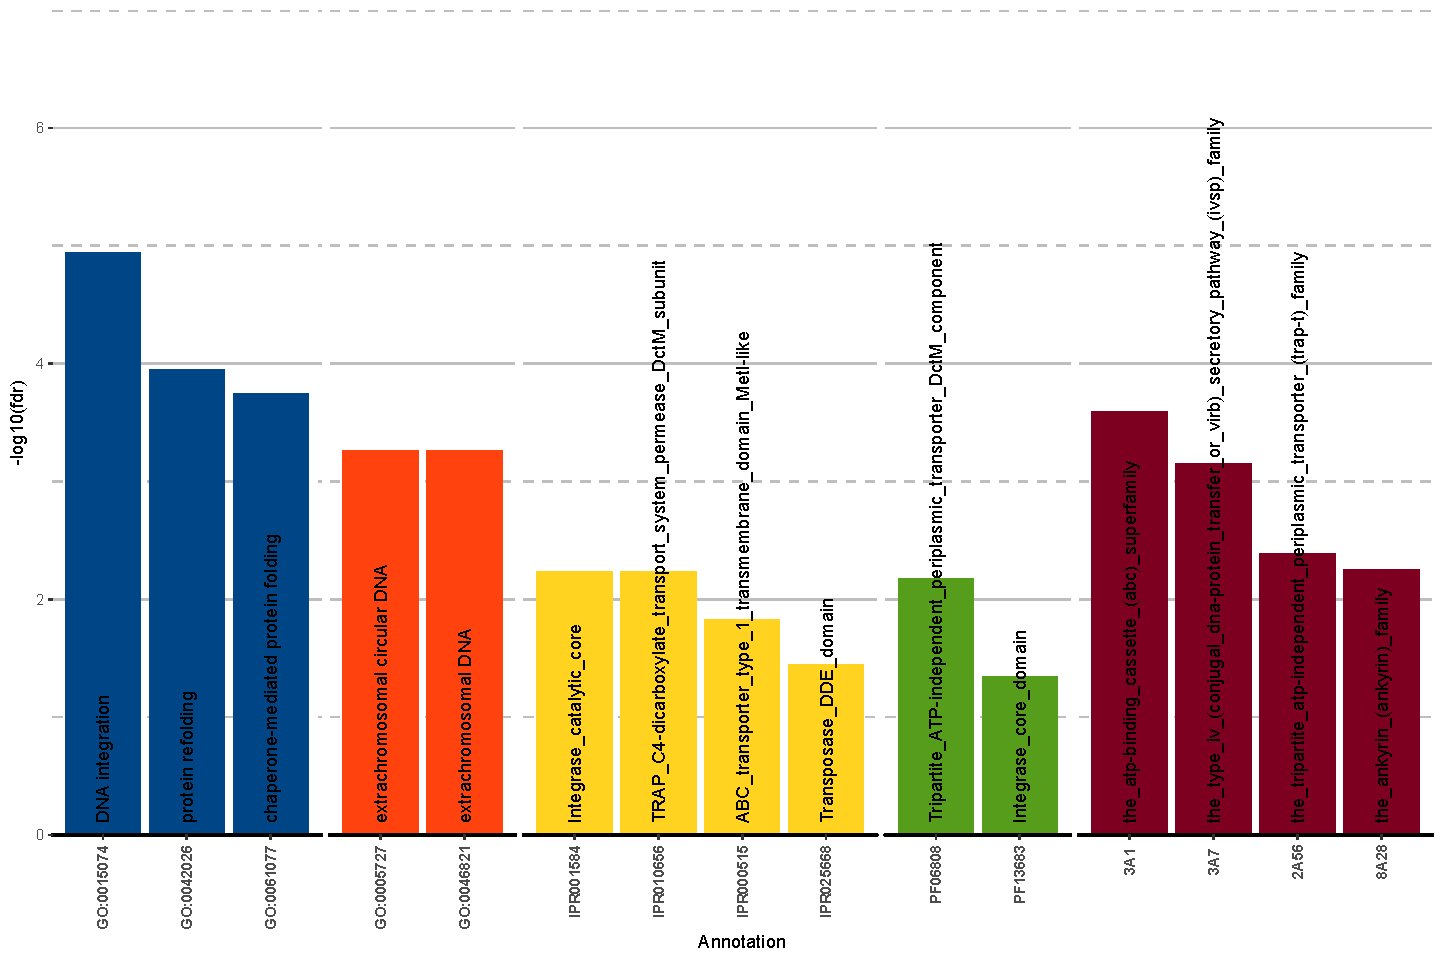
\includegraphics[width=\linewidth]{toPlot_specificToPhiSp.pdf}
    \caption{Graphical representation of the $-log_{10}(fdr)$ of the enriched categories in Cazy (Carbohydrate Enzyme Database), Gene ontology (GO), Inteproscan (IPR), Protein family (Pfam) and Transporter database (tcdb) in the set of {\phiSp}-specific genes. Functional categories related to Chitin degradation, Protein folding, Transport and DNA integration are overrepresented}
    \label{fig:spec}
\end{figure}


Proteinortho identified 1169 groups of orthologues present in all 13 species, 1091 genes specific to \phiSp{} and 2362 genes specific to \phiScl{}. The genes specific to \phiSp{} are enriched in functional terms related to protein refolding (GO:0042046, GO:0061077, HSP20, HSP70, HSP90, Clp, DnaJ.HSP40), DNA modification (GO:0015074, GO:0005727, GO:0046821, IPR01584, IPR025668, PF13683, GO:0005727, GO:0046821, TCDB 3.A.7), Tripartite ATP-independent periplasmic (TRAP) and ATP-binding cassette transporter (IPR010656, IPR000515, TCDB 3.A.1, 2.A.56) as well as  Chitin degradation (Cazy:GH23) (See Figure~\ref{fig:spec}). TRAP transporters were shown to mediate the uptake of compatible solutes in \textit{Halomonas elongata}~\cite{Grammann2002}, while the proteins related to refolding are known to be involved in stress-response~\cite{Verghese2012}  


In \phiScl{} the set of species specific genes are functionally enriched in terms related to protein folding, heat shock protein 70 and helix-turn-helix (HTH)-binding domain protein (see Supplementary Figure 1 and Supplementary Table).  The helix-turn-helix binding-motif is found in many proteins involved in gene expression regulation~\cite{Brennan1989}. 

\subsection{Gene family evolution}

\begin{figure}[htbp]
  \centering
  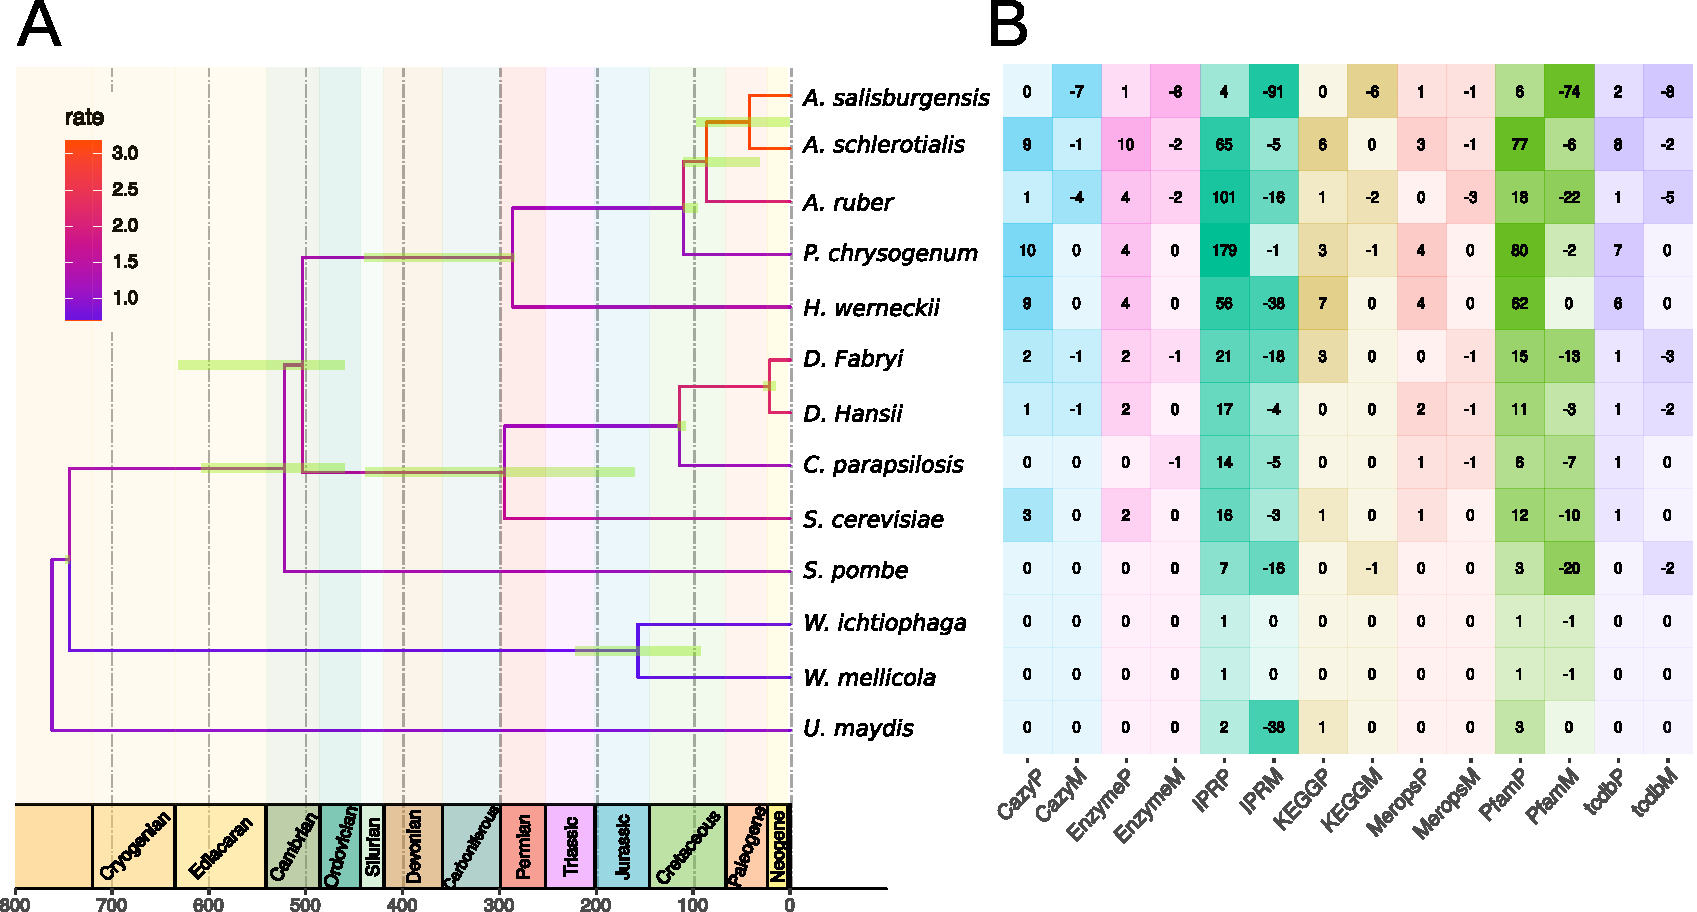
\includegraphics[width=\linewidth]{./geophyloTreeCAFE.pdf}
  \caption{\label{fig:gainLossTree} Phylogenomics analyses. A) Timetree generated from the merged alignment of the one-to-one homologues of the 13 species. The green bars represent the 95$\%$ confidence interval. Geologic periods are color-coded and  indicated at the bottom of the tree. Evolutionary rate is color encoded. B) CAFE analysis of the expansion and contraction of the annotation elements KEGG, Cazy, tcdb, Enzyme and Merops for the 13 species. The suffix M,P after the annotation categories stands for contraction and expansion, respectively.}
\end{figure}


A timetree for the 13 fungi was constructed from the multiple sequence alignments of the proteins shared by all strains and from 9 time anchors extracted from the TimeTree database~\cite{Kumar2017}(See Figure~\ref{fig:gainLossTree}). It is consistent with the currently accepted taxonomy~\cite{Kumar2017}. \phiSp{} and \phiScl{} separated approximately 41MYA(+/-40MYA), 20MY before the split between \debFab{} and \debHan{} and 40 MY after the split between \phiSp{}, \phiScl{} and \aspRub{}. Interestingly \phiSp{} and \phiScl{} exhibit the largest evolutionary rates, followed by the two \textit{Debaryomyces} species. 

This tree was used to estimate the numbers of rapidly evolving annotation elements with CAFE~\cite{DeBie2006}. The functional annotations used were derived for the carbohydrate enzymes (Cazy)~\cite{Cantarel2009}, general enzymes from the EggNog annotation~\cite{HuertaCepas2016}, Interproscan protein domains (IPR) ~\cite{Jones2014a}, KEGG pathways~\cite{Ogata1999}, proteolytic enzymes (Merops)~\cite{Rawlings2014}, Pfam protein domains~\cite{Finn2014a} and transporters from TCDB~\cite{Saier2006}. 

The internal node with the largest numbers of rapidly evolving annotation families is the one leading to the common ancestor of \textit{Hortaea} and \textit{Aspergillus} (\textit{leotiomyceta}) (See Supplementary Table 1). CAFE reports 106 IPR and 105 Pfam rapidly evolving families. The most significantly expanding families are related to fungal-specific transcription factors (p-value 4.75e-19) and Cytochrome P450E (p-value 1.127e-16). Cytochrome P450 was also shown to improve salt tolerance in plants~\cite{Yan2016} and is upregulated under salt stress in the fungus~\textit{Piriformosa indica}, a plant endophyte that confers salinity stress tolerance in rice plants~\cite{Gahlot2015}. 
%%Cytochrome P-450 is a large and diverse group of enzymes found in all kingdoms of life having monooxygenase and oxidoreductase activity, electron carrier activity and acting on paired donors, with incorporation or reduction of molecular oxygen. The substrates of cytochrome P-450 enzymes include metabolic intermediates such as fatty acids and lipids. In addition, 
%%Cytochrome P-450 gene is known to play a role in salt tolerance in fungi, as Piriformospora indica, a root endophytic fungus ~\cite{Gahlot2015}. This fungus colonizes the roots of plants and provides tolerance to abiotic stress in the plants, such as salt stress ~\cite{Gahlot2015}.
An additional significantly expanding family was DUF3468 (DUF, domain of unknown function, p-value 1.59e-15), a protein domain involved in transcription activation of genes related to asexual conidiation and sexual differentiation in \aspNid{} and \textit{Aspergillus flavus}~\cite{Chang2013}.

%factor involved in sexual and asexual reproduction~\cite{} DUF3468 is a domain of the C6 zinc cluster DNA-binding proteins. The zinc-binding proteins form one of the largest families of transcription factors in eukaryotes. They are categorized into three main classes based on their zinc finger binding motifs ~\cite{MacPherson2006}, namely (C2H2), (C4), and (C6). Only fungi and yeast contain the C6 zinc cluster DNA-binding proteins ~\cite{Chang2013}. 
%The roles of fungal C6 proteins as well as of the unique domain DUF3468, are still in its infancy~\cite{Chang2013}, but it has been reported that in \textit{A. flavus} 7$\%$ of C6 proteins contain a DUF3468 domain. Two \textit{A. nidulans} C6 proteins containing the DUF3468 are involved in asexual conidiation and another two in sexual differentiation ~\cite{Chang2013}.

The branch leading to \phiSp{} exhibits the largest contraction of gene families from all species analyzed: 91 IPR, 74 Pfam, 7 Cazy, 8 tcdb, 1 Merops and 8 Enzyme families contracted significantly in line with the reduction in genome size of 27$\%$ compared to to \phiScl{}. Fungal transcription factors (PF11951) exhibit the largest loss in \phiSp{} (-17). Protein families transporting amino acid and oligopeptide (2A3, -11; IPR002293,-9; 2A18, -5; PF03169, -3), fatty acid (4C1, -7) and iron (2A108, -5)  are contracting in \phiSp{}.
Interestingly the amino acid polyamine organocation superfamily (APC) contracted also in \aspRub{} (2A3, -8). It is one of the largest families of secondary active transporters and it is found in all leaving organisms~\cite{Paulsen2000}. Another family depleted in both \phiSp{} and \aspRub{} is the  aminoglycoside phosphotransferase, a bacterial antibiotic resistance protein (IPR002575) with a reduction of 15 and 13 members, respectively. 
%In some halotolerant bacteria, as \textit{Aphanothece halophytica}, it has been reported that the presence of a sodium-dependent transporter is involved in the uptake of glycine and glutamine. \textit{Aphanothece halophytica} accumulates a large amount of glycine betaine (betaine) under high-salinity conditions. In this bacterium, betaine is synthesized by a three-step methylation of glycine. Therefore, the synthesis and uptake of glycine are indispensable ~\cite{Bualuang2015}. 
%\aspRub{} shows a high number of both contractions and expansions in Pfam (+16 and -22) but an especially high number of expansion in the IPR database (101). In contrast, the other halophilic fungus \walIch{} harbors only one family with a significant size change.

A few annotation families expanded in \phiSp{}. These families are related to the type IV secretory pathway, which exports proteins or DNA-protein complexes out of the cell~\cite{Saier2007}  (3A7 +9), the TRAP-C4 transporter (IPR010656 +6, PF06808 +6), the fungal cellulose binding domain (PF00734, +5), the integrase catalytic core (IPR001584), cutinase (PF01083), sodium:bile-acid symporter/arsenical resistance protein Acr3 (PF01758 +2) and secretory lipase (PF03583 +2). The increase in cellulose degrading ability due to fungal cellulose binding domain~\cite{Gilkes1991} and cutinase~\cite{Sweigard1992} is probably related to the environment, a wooden staircase, from which  \phiSp{} was isolated. In yeast, proteins belonging to the PF01758 family confer arsenic resistance by extrusion of sodium arsenate and sodium arsenite~\cite{Fu2009}

\subsubsection{Gene Family Enrichment}

The significance of size variations of functional annotations families were studied  by comparing species or group of fungal species (See Table~\ref{tab:species}) with the help of chi-squared tests.
The most significant bias were seen for the MFS transporters, which showed a peculiar pattern of enrichment. \phiSp{} has significantly more MFS (2A1, IPR020846) transporters than \walIch{}, but significantly less than \phiScl{} and \aspRub{} (See Figure~\ref{fig:ovun} and Supplementary Table 1). Further there are significantly more MFS transporters in halotolerant fungi than in the halophiles (fdr=0.018). Still compared to the group of salt intolerant fungi both the halophiles (fdr=3.76$e^{-15}$) and the halotolerant(fdr=7.19$e^{-37}$) are enriched in MFS. 

Genes involved in protein translation, like ribosomes (GO:0003735, GO:0005840), RNA binding (GO:0003723)  reverse transcriptase (GO:013103, GO:0015074) are depleted in halophiles and halotolerant compared to the control group. In contrast, terms involved in transcription like RNA polymerase II (GO:0000981), transcription (GO:0006531, GO:0006535), transcription factor (IPR007219, IPR001138) are enriched in both H and HH compared to control. Terms related to cytochrome P450 E-class group I (GO:0016491, GO:0055114,IPR001128, IPR023753, IPR002401, IPR017972) are enriched in both groups of salt resistant fungi compared to the control group. 

\begin{figure}[htbp]
    \centering
    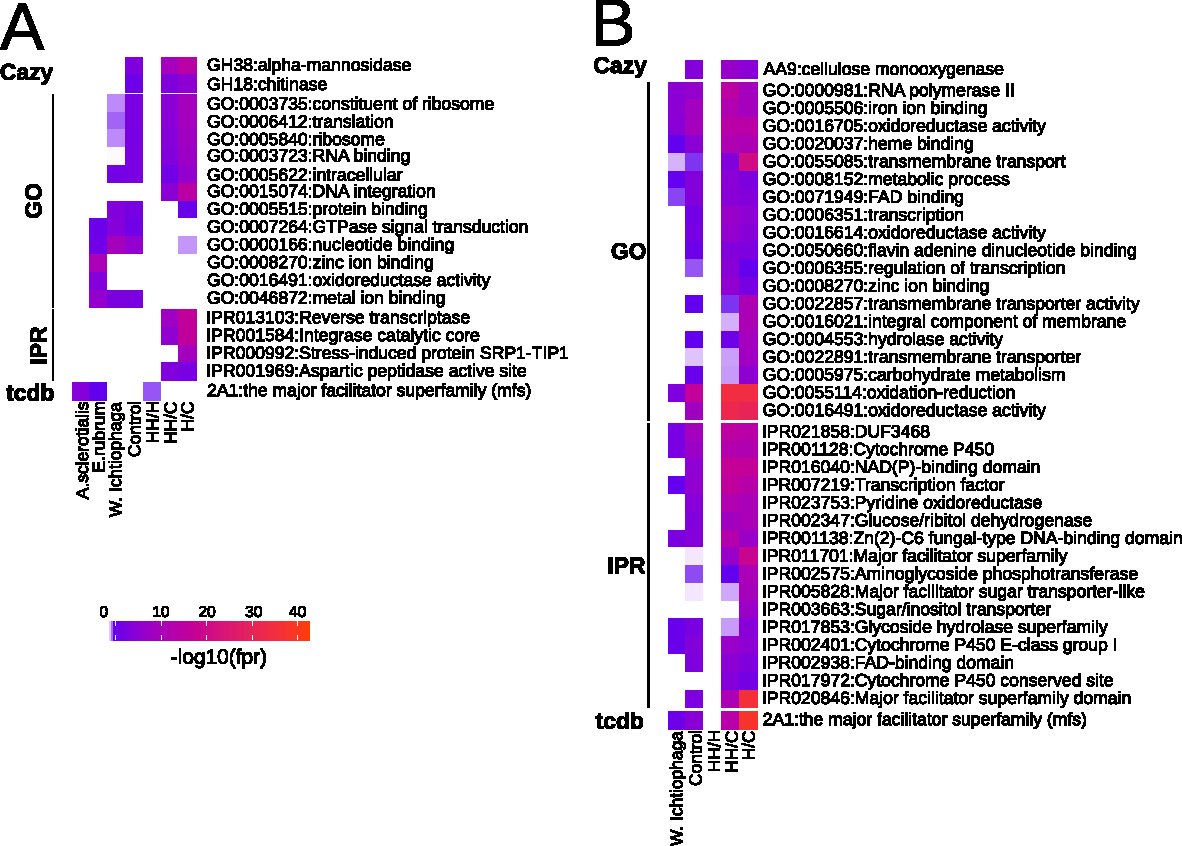
\includegraphics[width=\linewidth]{over_under_final.pdf}
    \caption{\label{fig:ovun} Heatmap of the $-log(fdr)$ of the significantly enriched or depleted functional annotations in {\phiSp} compared to  {\phiScl}, {\aspRub}, {\walIch}. Depletion/enrichment found in HH vs H, HH vs C and H vs C are also shown. Only entries with an enrichment/depletion with an fdr$<1e^{-5}$ are shown. \textbf{A} Depletion \textbf{B} Enrichment.
    }
\end{figure}

\subsection{Amino acid composition}
The protein amino-acid (AA) composition of the C,H and HH groups for the set of orthologous genes and for the set of exported proteins, i.e. containing a Signal-P annotation, was compared  (See Figure~\ref{fig:AABIAS} and Supplementary Table 1). With respect to the control group, the conserved proteins in halophile fungi are significantly enriched in Glycine, Proline and Arginine and depleted in Isoleucine and Lysine (See Figure~\ref{fig:AABIAS}A). The same bias pattern for those 5 AA was previously reported in the extremely halophile bacteria \textit{Salinibacter ruber} and \textit{Halomonas elongata} and the archaea \textit{Halobacterium salinarum}, \textit{Haloarcula marismortui} compared to \textit{Escherichia coli}~\cite{Oren2002}. A low occurence of lysines and increase of arginines in halophilic proteins is a signature of halophilic microorganisms~\cite{Paul2008,Tadeo2009}. Psychrophilic organisms, which similar to halophiles face reduced water availability, also exhibit an increased glycine protein content~\cite{De_Maayer2014}. 

Among the set of exported proteins, the acidic AA aspartate and glutamate are overrepresented in halophiles compared to the control group. This is a general characteristic found in many osmotolerant bacteria~\cite{Fukuchi2003, Paul2008}. This is similar to the trend found in conserved proteins, glycine and proline are enriched in proteins of the three studied halophiles. Finally the serine depletion was previously reported in halophilic archaea~\cite{Tadeo2009}.

\begin{figure}
    \centering
    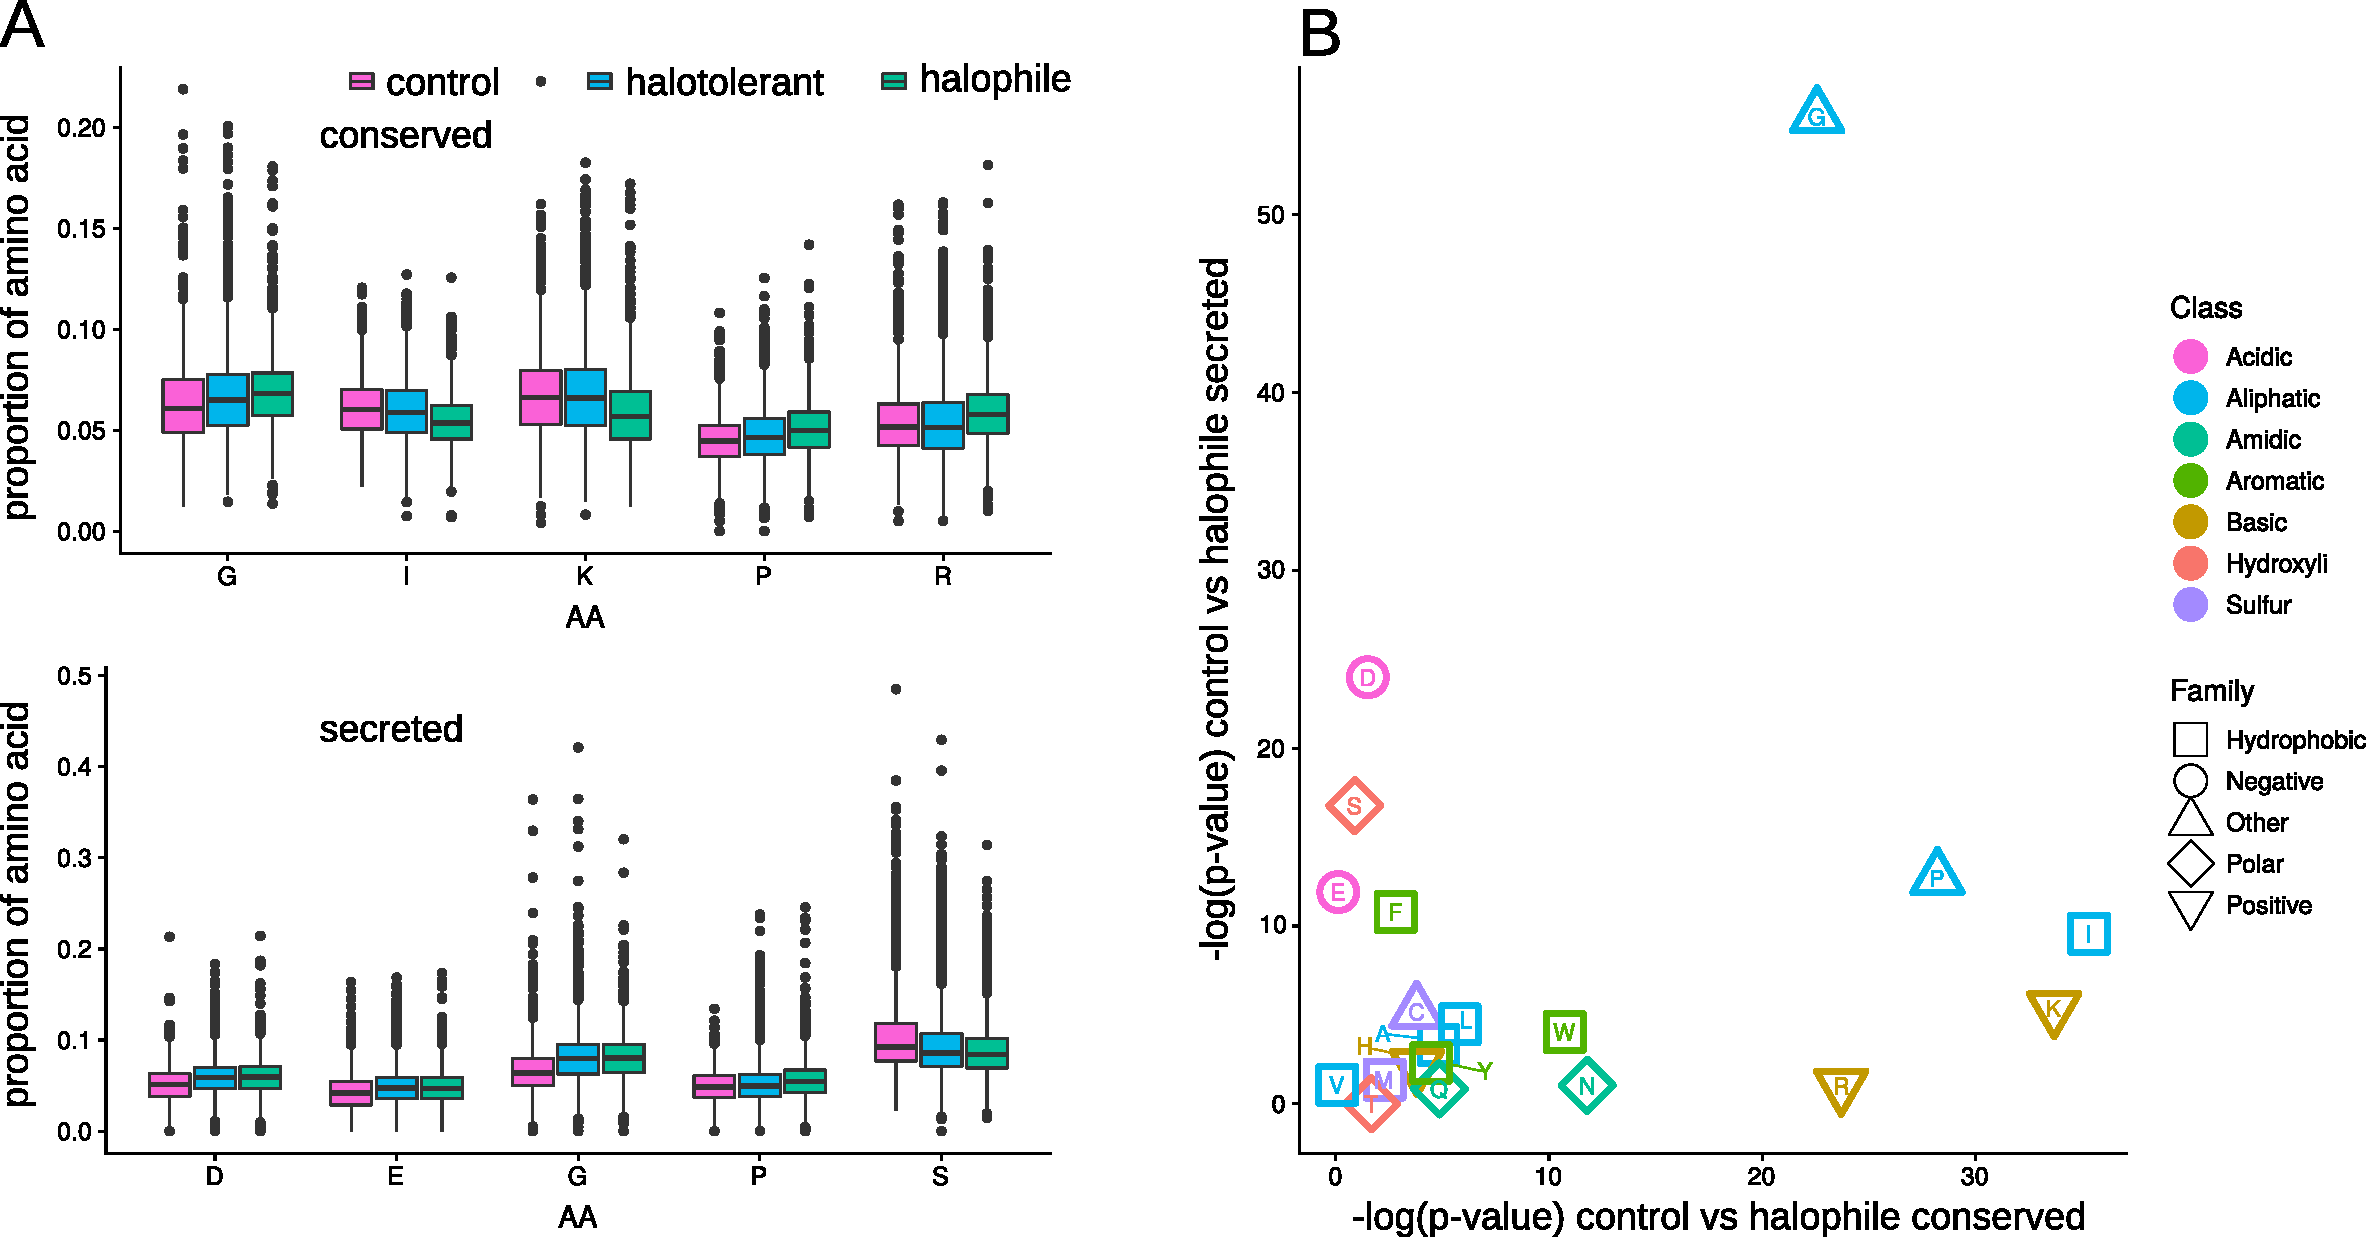
\includegraphics[width=\linewidth]{AAAnalysis.pdf}
    \caption{\label{fig:AABIAS} Bias in amino-acids (AA) distribution between the set of control, halotolerant and halophile fungi. A) Boxplot representing the distribution of AA for the 5 AA with the most significant bias between the control and halophile group for the set of conserved(top) and secreted proteins (bottom). B) Scatter plot of the $-log(p-value)$ computed with the wilcoxon-test for the AA distribution bias for the set of conserved proteins and the set of secreted proteins. }
\end{figure}

\subsection{Differential expression between 5$\%$ and 20 $\%$} NaCl
The differential expressions of genes between the low and high salt concentrations was studied. Upregulated genes are defined as the set of transcripts that exhibit an increase in expression at 20$\%$ salt concentration, while downregulated genes exhibit a reduced expression under high salinity.  

%The halotolerant fungus has to adapt a variety of cellular functions %to cope with the different  salt concentrations, and therefore its %growth is slower  at high salinities. On the contrary, our data show %that the halophilic strain exhibits  less changes on the %transcriptome level, since the fungus is growing in an environment %with a relatively constant high level of salt, optimal for its %growth, and therefore does not need adaptation mechanisms for rapid %changes in salinity. 
\subsubsection{\phiScl}

\begin{figure}[htpb]
    \centering
    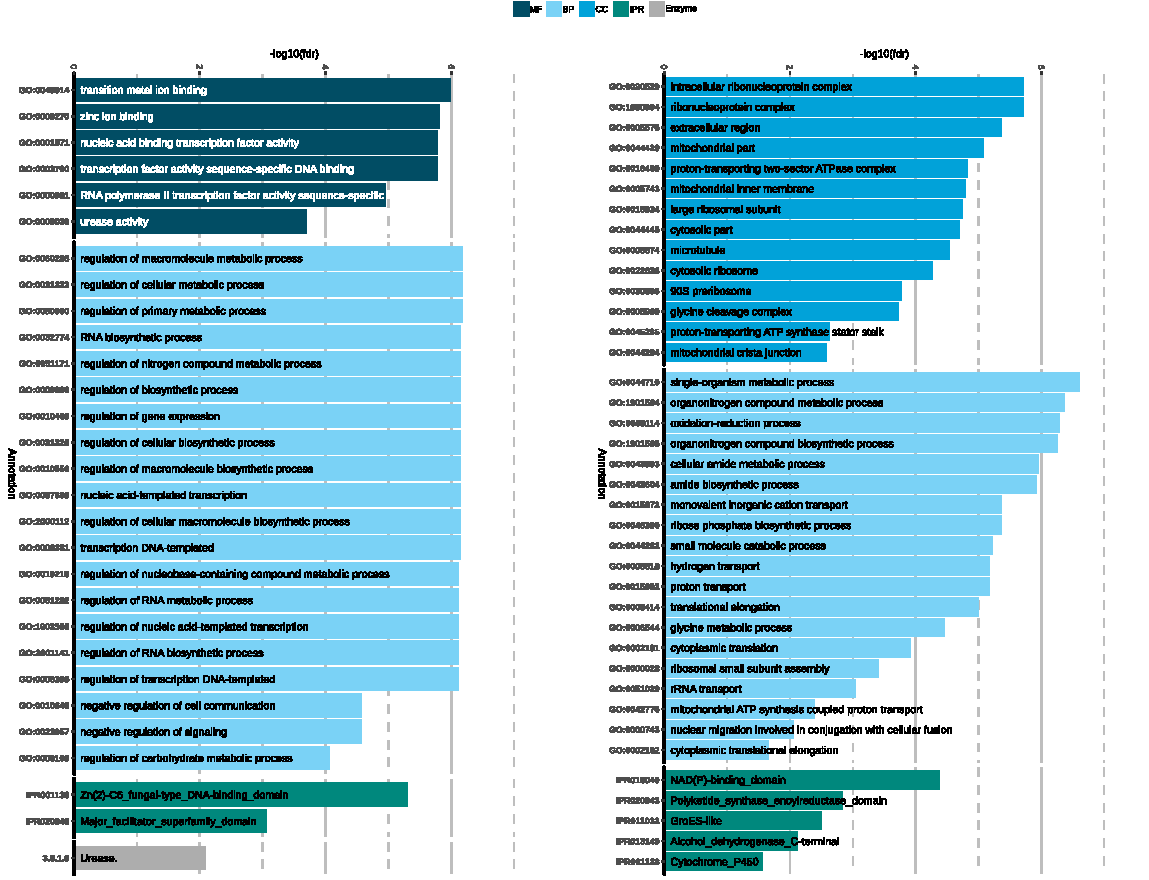
\includegraphics[width=\linewidth]{phiScl_SALT_summary.pdf}
    \caption{\label{fig:phiSclUpDown} Barplots showing overrepresented functional annotations in the set of regulated genes in {\phiScl}. \textbf{A} Enriched functional terms in the set of downregulated genes. \textbf{B} Enriched functional terms in the set of upregulated genes.}
\end{figure}

\phiScl{} differentially regulates 2097 genes (1121 up- and 976 downregulated fdr<0.05, $|log_{2}FC|$>1) between both salt concentrations. The most strongly upregulated gene (x3536) belongs to the Major facilitator superfamily (MFS) transporter, which are membrane transport proteins that facilitate movement of small solutes across cell membranes in response to osmotic gradients ~\cite{Pao1998}. Among the 96 genes upregulated by a factor larger than 50 in the halotolerant fungus, 14 genes are related to transmembrane transport (See Supplementary Table). Cerato-ulmin hydrophobin, a parasitic fitness factor of the agents of Dutch elm disease~\cite{Temple1997} is upregulated by a factor 2641. The regulation of this hydrophobin might indicate a role in salt resistance, as previously reported in \walIch{} ~\cite{Plemenitas2014}. Given the fact that the halotolerant strain is a dog pathogen, this hydrophobin might be involved in the strain pathogenicity~\cite{Sigler2010}.

The C-terminal dimerisation domain found in tranposases of elements belonging to the activator superfamily is increased by a factor 280 under high salt condition, indicating that DNA modification might take place. A similar feature was seen in sunflower exposed to salt and drought stress~\cite{Liu2003}. Transcriptional regulators are also found among the most upregulated genes~\cite{Shelest2017}. A gene involved in protein neddylation~\cite{Yashiroda2003}, has its expression increased by a factor of 1571.  Inositol monophosphatase, which is upregulated by a factor 571, is involved in the phosphatidylinositol signaling pathway and was shown to increase Na$^+$ resistance in yeast~\cite{Lopez1999}.  A F-box domain containing protein is upregulated by a factor 286 upon salt-induced stress, which is in line with previous reports in \schPom{}~\cite{Hermand2006}. Interestingly, two genes involved in the synthesis of antibiotics, Acyl-CoA 6-aminopenicillanic-acid-acyltransferase and pristinamycin IIA synthase subunit A are upregulated by factor of 369 and 338, respectively.

Among the genes downregulated by a factor larger than 50, eight are related to transporters and one is related to SAM-dependent methyltransferase. Chorismatase-degrading enzymes are downregulated, in agreement with salinity stress experiment in~\textit{Carthamus tinctorius}\cite{Sadeghi2013}, where chorismatase synthase was upregulated upon salinity stress, indicating that chorismate plays a role in salt resistance. Two cupredoxin are downregulated by a factor 247. A reverse transcriptase and a integrase are downregulated 95 and 129 times, respectively, while one Zn$_2$-Cys6 transcription factor is downregulated by a factor of 124.

The functional enrichment analysis for the downregulated genes indicates that transcriptional factors,  MFS transporters and urease activity (Enzyme 3.5.1.5 fdr=0.0083, GO:0009039 fdr=3.15e-4) are negatively impacted by the high salt concentration (see Supplementary Table 1 and Figure~\ref{fig:phiSclUpDown}). It was previously shown that a depletion of urease improves salt resistance in \textit{Arabidopsis thaliana}~\cite{Bu2015}.

For the set of upregulated genes, an enrichment in translation, glycine metabolism, oxidation-reduction process, mitochondrial ATP synthesis and microtubule is seen. Osmotic stress was previously shown to transiently increase the free glycine concentration in wheat~\cite{Kovacs2012}. The five upregulated genes related to microtubules are two tubulins (jg1358, jg9339), one kinesin (jg11911), one dynein (jg2827) and one cytoskeleton associated protein (jg228). These genes are involved in the transportation of vacuole and organelles along the microtubules~\cite{Vale2003}.
\subsubsection{\phiSp{}}
\begin{figure}[htpb]
    \centering
    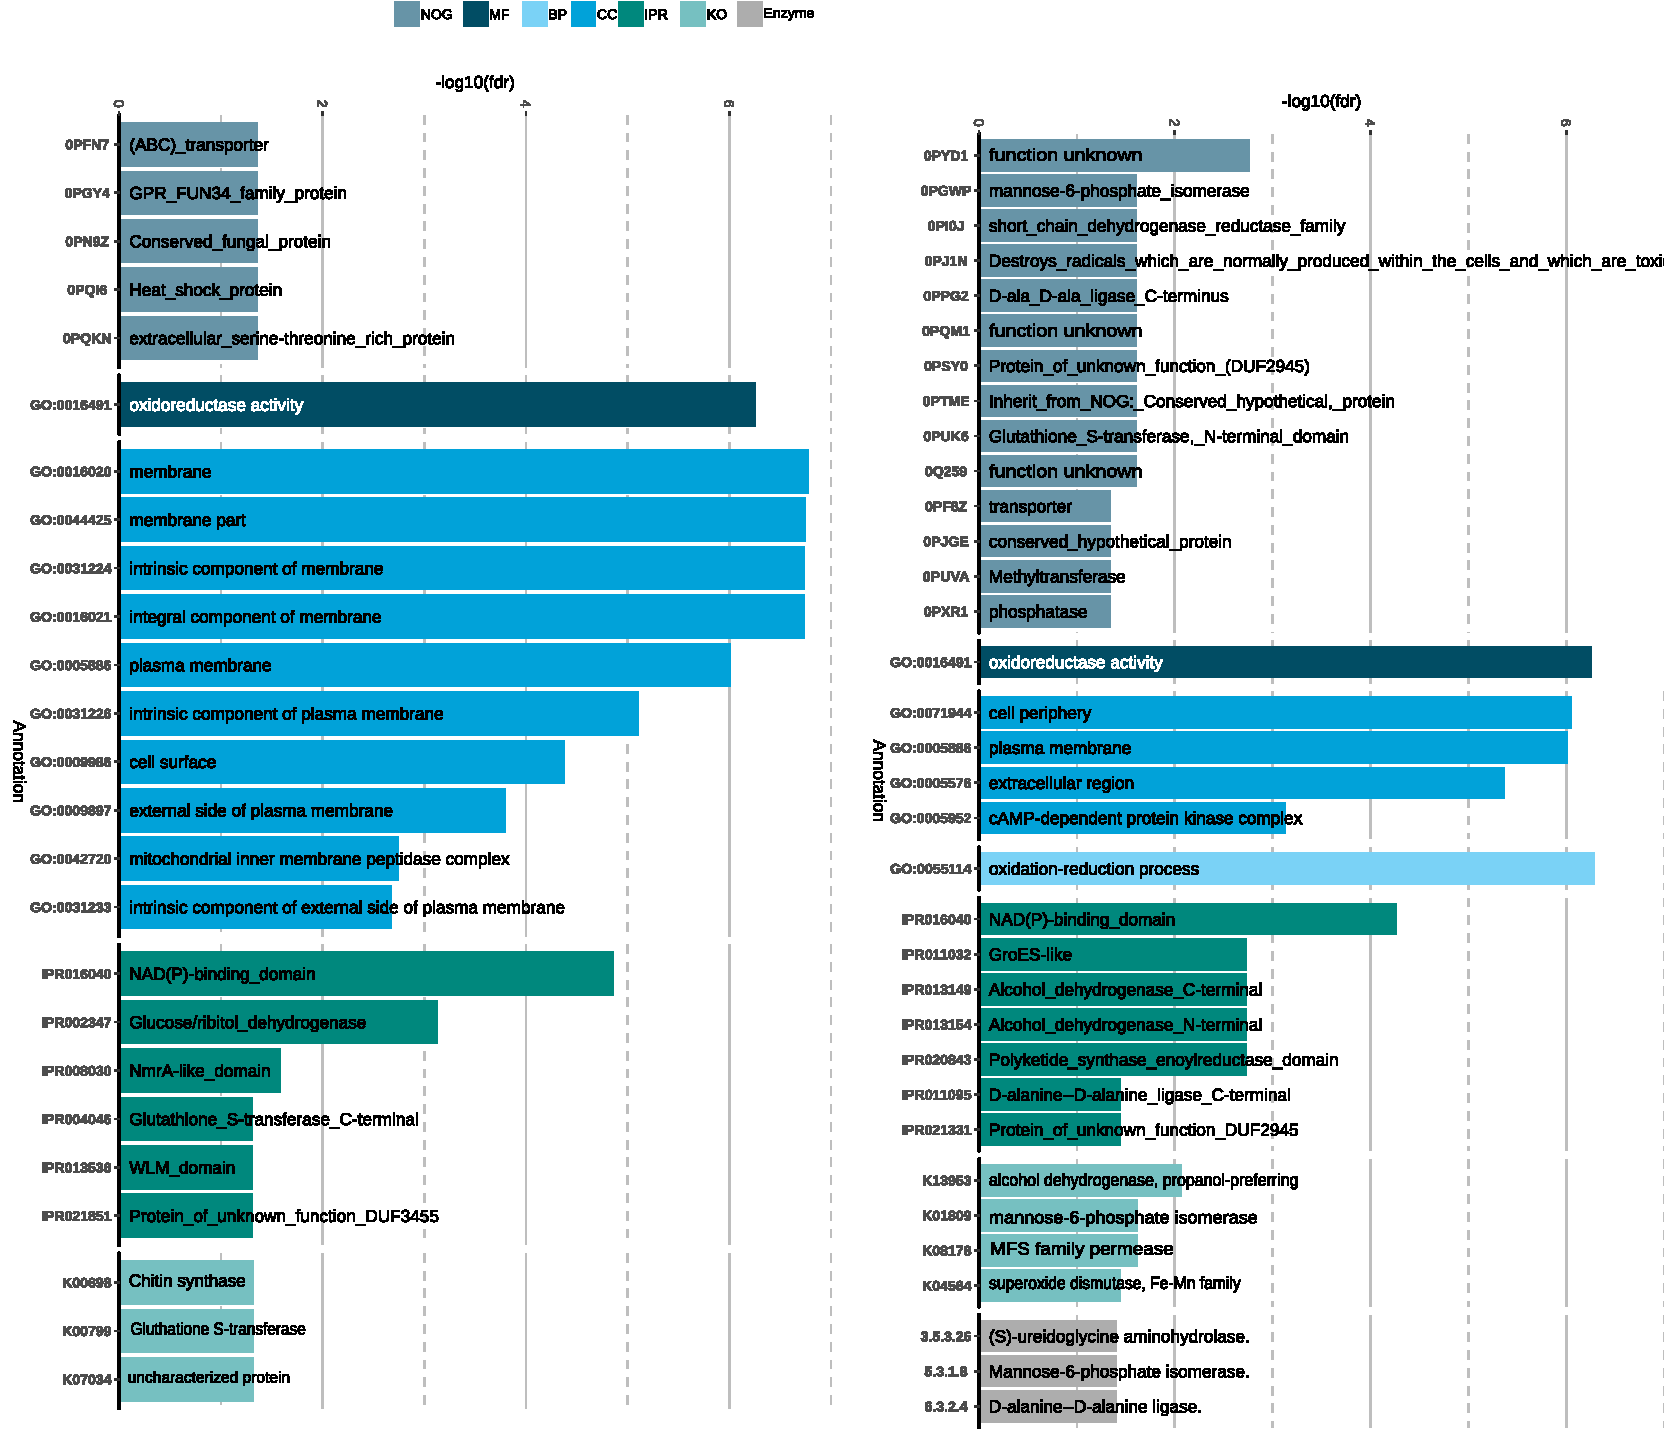
\includegraphics[width=\linewidth]{phiSp_SALT_summary.pdf}
    \caption{\label{fig:phiSpUpDown} Barplots showing overrepresented functional annotations in the set of regulated genes in {\phiSp}. \textbf{A} Enriched functional terms in the set of downregulated genes. \textbf{B} Enriched functional terms in the set of upregulated genes.}
\end{figure}

In \phiSp{} 305 and 306 gene were up- and downregulated, respectively. The most upregulated gene (x9013) is a peptidase S8 subtilisin protein with putative keratinolytic activity. Although the biological functions of most fungal subtilases are not yet described, some attempts led to the assumption that subtilisins (S8) could be related to a saprotrophic lifestyle~\cite{Leger1997}. More recently a study showed striking correlations for subtilisins (S8) expansion in pathogenic and soil/dung inhabiting fungi ~\cite{Muszewska2017FungalRepertoire}.  Subtilases have further been reported to be involved in drought and salt resistance mechanisms in plants~\cite{Liu2007}. An  example is the \textit{Arabidopsis thaliana} subtilase AtSBT6.1, which is associated with the unfolded protein response on salt stress through the cleavage of an ER-resident type II membrane protein (bZIP28). The cleavage of this protein is essential for the activation of genes associated with the salt stress response~\cite{Figueiredo2018}. 

Among the proteins with at least 50 fold upregulation, eight proteins are glycoside hydrolase, 3 are involved in oxido-reduction processes, 4 exhibit a cupin-like domain, 2 are involved in post-translational modification (See Supplementary Table). Among the set of genes downregulated at least 50 fold, 4 ribitol dehydrogenase, 7 transporters, two cyclic amino-acid related enzymes,  2 transcription factors and 2 alcohol dehydrogenase are found. 

Functional enrichment analyses of the downregulated genes indicates that the expression of membrane-located proteins, especially serine/threonine rich proteins are downregulated (See Figure~\ref{fig:phiSpUpDown} and Supplementary Table 1). Similarly Glutathione S-transferase, a gene previously shown to play a negative role in salt stress tolerance in \textit{A. thaliana}~\cite{Chen2012}, was downregulated under high salinity condition. Chitin synthase genes were downregulated in line with proteomic results in yeast~\cite{Szopinska2011}.

The set of upregulated genes covers a broader spectrum of functions than that of the downregulated genes. Genes located at the cell periphery and extracellular region are overrepresented in the set of upregulated genes (See Figure~\ref{fig:phiSpUpDown} and Supplementary Table 1). The overrepresentation of functional terms related to cell wall production like the D-alanine--D-alanine ligase and mannose-6-phosphate isomerase might indicate that cell wall damages are happening under high salinity~\cite{Ene2015}. Enrichment of superoxide-dismutase (K04564), which are enzymes involved in the catalysis of superoxide, is a known marker of oxidative stress and salt stress~\cite{Gostincar2018}. Finally the overrepresentation of MFS transporters is a paramount osmotic stress response, as these transporters are transporting small molecules in response to chemiomostic ion gradients~\cite{Pao1998}


\subsubsection{Comparative transcriptomics}
Difference and similarities in expression of genes found in both studied fungal strains were assessed. A total of 84 genes were 1-to-1 homologue in both strains and were significantly regulated. Genes upregulated in the halophile and halotolerant species were related to polyketide synthase, chloroperoxidase, haloacid dehalogenase, fructose-biphosphate aldolase, copper transport and pectinolytic enzyme (See Supplementary Table). Chloroperoxidase were shown to be potential chlorinators of lignin in plant materials and to contribute to lignin degration~\cite{OrtizBermudez2003}. This is similar to the use of chlorine for wood pulp delignification~\cite{dence1971halogenation}. In the fungi \textit{Fusarium fujikuroi} and \textit{Neurospora crassa} genes belonging to the haloacid dehalogenase family were shown to be involved in the osmotic stress and glycerol metabolism~\cite{Garcia-Martinez2014}. Conserved genes downregulated in both species are related to amino acid transport, trehalose-phosphatase, thiolase and the p53 transcription factor. 

Genes solely upregulated in \phiScl{} were related to oxido-reductive processes, Zinc transport and polyketide synthase. In contrast, genes upregulated in the halophile and downregulated in the halotolerant were related to the Cation/H+ exchanger, threonine/serine exporter, voltage-dependent channel, intradiol cleavage, the putative sensor protein SUR7/Rim9, which is a pH-response regulator protein,  and the isochorismatase, a gene involved in salycilic acid metabolism. The upregulation of the last gene only in the halophilic strain may indicate an adaptive advantage to survive permanently in a hypersaline environment. Salicylic acid (SA), is a natural phenolic compound known to control many physiological and biochemical functions in plants such as growth, development  and responses to abiotic stresses ~\cite{HaraM.FurukawaJ.SatoA.MizoguchiT.andMiura2012}. Some studies have shown that SA plays a role in the response to salinity  in plants, and that its exogenous application  improves tolerance to salt stress in several  species ~\cite{Miura2014}. 



\subsection{Comparison to fungal osmoadaptation and osmoregulation}
The literature on osmoadaptation and osmoregulation in fungi was compared to the genome content and transcription patterns of \phiScl{} and \phiSp{}. 

\subsubsection{Osmosensing}
All members of both branches of the high osmolarity signalling pathway were found in \phiSp{} and \phiScl{}~\cite{Hohmann2009,Ma2013}. Histidine Kinase 7A/B~\cite{Lenassi2007} from \horWer{}, the mitogen activated protein kinase (Kss1)~\cite{Mortimer1989} from \sacCer{}, both involved in signal transduction,  and the cell wall integrity sensor (MID2)~\cite{Ono1994} are found in the halotolerant but not in the halophile genome. Interestingly, the irritation of the cell wall and membrane by shrinking  triggers induction of the HOG signalling pathway e.g. in \textit{S. cerevisiae} ~\cite{Hohmann2002, Stratford2019}. Inversely, \phiSp{} has a homologue of the  Tyrosine-protein phosphatase 3 (Ptp3), which is involved in the repression of the Hog1 gene~\cite{Wurgler-Murphy1997} (See Supplementary Table).

Protein kinase A (PKA1, TPK1), an enzyme generally involved in the regulation of the glycogen, sugar and lipid metabolism that negatively regulates the transcription factors Msn2/Msn4~\cite{Smith1998} is upregulated six fold in \phiSp{} but downregulated by a factor of three in \phiScl{}. Tor1, another gene that negatively regulates the Msn2/Msn4 transcription factors~\cite{Smith1998} is also downregulated by a factor 5 in \phiScl{} but not in \phiSp{}. The MAP kinase kinase Pbs2, which is involved in the HOG pathway, and Gsp2, a histidine kinase involved in the nuclear import of Hog1~\cite{Ferrigno1998}, are upregulated 5.5 and 4.8 fold at high salt concentration in \phiScl{} but not in \phiSp{}. Nik1, a histidine kinase involved in the Sln1 branch of the HOG pathway~\cite{Kruppa2006}, is downregulated 9 fold in \phiScl{}.

\subsubsection{Ion homoeostasis}
The genome of \phiSp{} contains most of the ion transporter reported to be involved in ion trafficking during osmotic stress in \sacCer{} and \horWer{}, with the exception of the high affinity potassium transporter (Hak1)~\cite{Kruppa2006}, the potassium antiporter (Kha1)~\cite{Plemenitas2014} and the outward-rectifier potassium channel Tok1~\cite{Plemenitas2014}. In \phiScl{} the endosomal/prevacuolar sodium/hydrogen exchanger (Nhx1) and Hak1 are missing. Tok1 and the mitochondrial exchanger system, while present in the halotolerant strain, are downregulated  four fold  at 20$\%$ NaCl in this strain. Pam1, a proton ATPase involved in salt resistance in \debHan{}~\cite{Prista2005} is upregulated by a factor of 13 in \phiScl{}. Similarly Nha1, the Na+/H+ antiporter is upregulated 6.3 fold under high salt concentration. In the obligate halophile ENA1, a  P-type ATPase sodium pump involved in Na+ and Li+ efflux~\cite{Haro1991} is upregulated by a factor of 39. 

\subsubsection{Cellular respiration}
In \phiScl{} seven genes annotated as involved in respiration (GO:0045333) are upregulated under high salt concentration. The electron carrier protein Cyc1 is upregulated by a factor 4.62, the cytochrome b-c1 complex subunit 7 (Qcr7) expression increases by a factor 3.94 and the cytochrome c oxidase subunit VIa (Cox13) is induced by a factor of 3.63. Further a ADP/ATP carrier protein (Aac) is upregulated by a factor of 6.14. Mitochondrial Isocitrate dehydrogenase (Idh1), malate dehydrogenase (Mdh1) and mitochondrial trans-2-enoyl-CoA reductase are upregulated 4.82, 12.82 and 4.62 fold. This strongly indicates that the ATP production is increased during salt stress in the halotolerant strain. In contrast, no genes related to cellular respiration were significantly regulated in \phiSp{}.

\subsubsection{Stress response}
 \phiScl{} has a stress response more pronounced than \phiSp{}, both in terms of the number genes regulated as well as the regulation intensity.
 Markers of oxidative stress response are strongly upregulated in \phiScl{} at high salt concentration, in line with the increased respiratory process seen in the halotolerant strain. 
  The mitochondrial superoxide dismutase (SOD2), an important antioxidant defense, catalyzes the dismutation of superoxide $O_2^-$, a mitochondrial byproduct of respiration, into oxygen and hydrogen peroxide. This gene is upregulated by a factor 8.3 in \phiScl{} at high salinity. H2O2 is then reduced to H2O by Peroxiredoxin (Prx1) using electrons from the reduced form of thioredoxin (Trx)~\cite{Pannala2015}. In \phiSp{} Trx is upregulated by a factor 3.6 at 20$\%$ salt concentration. Two mitochondrial Prx1 are upregulated by 9.5 and 6.5 fold, respectively. Further the nuclear thioredoxin peroxidase DOT5 and the AHP1 peroxiredoxin are upregulated by a factor 4.8 and 5.9, respectively.  H202 can also be scavenged through the glutathione system with the help of glutathion redoxins (Grx)~\cite{Pannala2015}. A homologue to Grx1 and Grx2 and a homologue to Grx3 and Grx4 are upregulated 6.31 and 4.3 in \phiScl{}, respectively. Further, two catalase paralogues (Ctt1), an enzyme that is involved in peroxide scavenging, are upregulated by a factor 10.1 and 6.9, respectively. The homologue to MCA1, a regulator of apoptosis upon H2O2 and clearance of insoluble protein aggregates is upregulated by a factor 3.71~\cite{Madeo2002,Lee2010}. Additional studies have shown that oxidative stress originating from intensive mitochondrial respiration ~\cite{Gille1995} can pose a further threat to the survival of aerobic microorganisms living in high-salinity environments. Therefore, this stress can be one of the limiting factors for growth in such environments. In the halotolerant strain \horWer{}, the levels of ROS degradation and resistance determine the upper limit of salt tolerance ~\cite{Petrovic2006}.  The peptidyl-prolyl cis/trans-isomerase, a gene involved in protein folding~\cite{Guo2014} undergo an upregulation under salt stress by a factor of 3.43 in the halotolerant strain.

 
 In \phiSp{} the oxidative stress response is moderate. Similar to the halotolerant strain, Ctt1 is upregulated by a factor 8.8. Methionine sulfoxide reductase (Mxr2), a gene protecting against methionine oxidation by catalyzing thio-dependent reduction of oxidized meth residues~\cite{Stadtman2003}, saw a 5.29 fold increase in transcription. Interestingly, the obligate halophile reduces the production of superoxide radicals by downregulating NADPH oxidase and the NADPH oxidase regulator by a factor 5 and 10, respectively. Beyond genes involved in oxidative stress response, \phiSp{} upregulates HSP12, a chaperone regulated in osmotic stress conditions in~\sacCer{}, by a factor of 5~\cite{Saito2012}.  

  
\subsubsection{Cell interface}

In the extracellular region, \phiSp{} strongly upregulates the subtilisin peptidase (S8 x8964), two cellulose degradation enzymes (GH51, x62), a pectinolytic enzyme (EC:4.2.2.2 x23) and a cellulase (GH5 x22.62). Together with the upregulation of a chloroperoxidase, that might be involved in the degradation of lignin, and the environment where this fungus has been isolated, i.e. a wooden staircase in a salt mine, it seems reasonable to assume that salt triggers a cellulolytic response in the obligate halophile. \phiScl{} strongly upregulates a hydrophobin (PF06766 x2646).

In the cell wall of the halotolerant fungus a beta glucosidase involved in cell wall remodeling (Uth1)~\cite{Kuznetsov2013} is upregulated by a factor 17, while a membrane bound HSP70 involved in selective cation trafficking is upregulated by a factor 6.33~\cite{Arispe2000}. In the halophilic fungus a lysophospholipase, an enzyme involved in phospholipid degradation and previously reported to be upregulated in \textit{Dunaliella salina} under high salt concentration~\cite{Katz2007}, saw its expression increases 18 fold.

At the membrane level besides the previously discussed transporters,  \phiScl{} increased the expression of a putative ammonia transporter (PKC1 x22.31), a dipeptidase (DPE1, x9.91), the Sur7 membrane protein involved in membrane organization and cell wall stress~\cite{Douglas2012} (x7.78), a sulfate permease (SulP x6.77) and a cellulolytic enzyme (EggNog: 0PG84 x11.15).
The halophile strain increases the transcription of two Guanine nucleotide proteins (G protein)~\cite{Vogler2008} (ion-translocating rhodopsin x10.63, Rheb x4.00) and one G protein-coupled receptor-like Gpr1 (x12.46), a gene involved in endocytosis, the Eisosome component PIL1/LSP1 (x32.11)~\cite{Walther2006} and two Sur7 membrane proteins(x4.37, x25.73).


\subsubsection{Compatible solute management}
 Known genes involved in compatible solutes management from halotolerant and obligate halophilic fungi were reviewed. Compatible solutes are known to be accumulated or synthesized during changed osmotic conditions.  One of these is D-mannitol, which can be synthesized by a reduction of fructose, catalyzed by NADP-dependent mannitol dehydrogenases~\cite{Zajc2013}. In \phiSp{} two homologues of NADP-dependent mannitol dehydrogenases are found in the genome but are not regulated in salty conditions while one homologue is found in \phiScl{} and is upregulated by a factor of 29. Still \phiSp{} upregulates Gre3, an aldole reductase involved in polyol metabolism~\cite{Saito2012} by a factor 28.
 
Three homologues genes of  Stl1, a glycerol/proton symporters of the plasma membrane,  are found in \phiSp{} and one in \phiScl{}. In comparison, four homologues were found in the genome of the obligate halophile fungi \walIch{}~\cite{Plemenitas2014}. In \phiSp{}, one copy of the genes is upregulated by a factor 8 and in \phiScl{} Stl1 is upregulated by a factor of 91. In \sacCer{} it was reported to be upregulated during hyperosmotic shock~\cite{Ferreira2005}. The aquaglyceroporin channel Fps1, which is opened in hypoosmotic conditions to release glycerol\cite{Luyten1995}, does not receive any regulation in \phiSp{} and is downregulated in \phiScl{} by a factor 30.

Glycine betaine is an osmoprotectant found in plant, animals, bacteria and fungi that is also involved in reactive oxygen scavenging~\cite{Lambou2013}. In \aspFum{}, glycine betaine is produced by converting first choline to betaine aldehyde with a choline oxidase. Betaine aldehyde or its rapidly forming hydrated equivalent gem-diol-choline are then converted to glycine betaine with the help of betaine aldehyde dehydrogenase or choline oxidase, respectively~\cite{Lambou2013}. In \phiSp{} two choline oxidase and one betaine aldehyde dehydrogenase are found while in \phiScl{} two copies and one copy are found, respectively. While \phiSp{} did not significantly regulate these enzymes, \phiScl{} increased the transcription of betaine aldehyde dehydrogenase by a factor of 4.5 in high salinity condition.

Genes involved in polyols metabolism  are also strongly upregulated. Polyols - also called sugar alcohols - compensate  for differences between the extracellular and intracellular water potential without affecting the integrity and function of proteins ~\cite{Brown1990}. In \phiScl{} gene jg11062 belongs to the same group as the L-arabitol 4-dehydrogenase from \aspFum{} and is upregulated by a factor of 1063 at high salt concentration (See Supplementary Table). A sorbitol dehydrogenase and a ribitol dehydrogenase are upregulated by a factor 62 and 67, respectively. The important role of polyols - and non reducing sugars as trehalose - for the resistance of extremotolerant fungi under osmotic stress was already described by Sterflinger ~\cite{Sterflinger1998}. However, this general protection strategy is widespread also in bacteria and archaea ~\cite{Gunde-Cimerman2018}.   

In the halotolerant strain, four SAM-dependent methyltransferase saw an increase in transcription by a factor 455, 218, 205 and 52 respectively,  similar to previous reports in algae~\cite{Krell2006}, where sequence homologue of the SAM-dependent methyltransferase are involved in the production of the compatible solute homoserine betaine~\cite{Pade2016}. Glutamine synthetase is upregulated by a factor 181, indicating that \phiScl{} might use glutamine as an osmolyte, something previously reported for \textit{Halobacillus halophilus}~\cite{Saum2006}. 

\section{Conclusions}
In this work the genomic adaptation and gene regulation of the obligate halophile~\phiSp{}, a fungus isolated from a wooden staircase in a salt mine, an extreme habitat with high salt concentrations, absence of light and reduced food availability, was studied by employing comparative genomics and transcriptomics approaches. The halotolerant pendant \phiScl{}, a dog pathogen, was used to gain insights into the environment-specific osmoadaptation and regulation of the obligate halophile. 

On the genomic level, \phiSp{} exhibit a 27$\%$ decrease in genome size and gene content compared to \phiScl{}. Considering the unique, extremely stable niche where the obligate halophile has been found, it can be hypothesized that the fungus optimized its genome content by dumping genes unnecessary for its survival, a known phenomenon in bacteria~\cite{Stepkowski2001}. Niche adaptation is further seen in the enrichment of genes involved in cellulose degradation. Halophile specific depletion of MFS transporters previously reported in \walIch{} and \aspRub{} ~\cite{Plemenitas2014,Kis-Papo2014-dn} was also found in \phiSp{} and might therefore be a strategy to survive in the stressful environment. This study further confirmed the specific amino-acid enrichment and depletion patterns found in other halophilic species compared to salt intolerant species.

The fact that the obligate halophile regulates three time fewer genes than the halotolerant strain between both salinities further underlines the adaptation of the former to high salt concentration. Besides the regulation of a few transporters like ENA1, STL1, a hydrophobin and an aldol-reductase, a gene reported to be involved in the production of compatible solutes, there is almost no sign that reveals that the obligate halophile is under stress at 20$\%$ salt concentration. Instead, the strong cellulolytic response is a strong indication that the high salt concentration is beneficial to \phiSp{} as it triggers the expression of a battery of wood degrading enzyme. Among them the chloroperoxidase is making use of the chloride ion to chlorinate lignin and improve its degradation, similar to the use of chlorine for wood pulp delignification. 

In contrast, the halotolerant strain exhibits both an osmotic- and oxidative-stress response. The link between both stresses  might probably be found in the respiration processes. In fact, it is probable that under high salinity, homeostatic regulation requires an increased supply of ATP, which is produced mainly from the respiration. At the transcriptome level the increased respiration is seen in the upregulation of genes involved in the electron transport chain and the citrate cycle. ROS originating from the respiration induces an oxidative stress response, as can be seen from the increased transcription of genes involved in oxidative-stress like superoxide dismutase, thioredoxin peroxidases, glutathione oxidoreductases and catalases. \phiScl{} further upregulates a hydrophobin, a family of protein that plays a role in salt resistance in \walIch{} and in pathogenicity.


%%%%%%%%%%%%%%%%%%%%%%%%%%%%%%%%%%%%%%%%%%


%%%%%%%%%%%%%%%%%%%%%%%%%%%%%%%%%%%%%%%%%%
\funding{This research was funded by the BOKU-VIBT Equipment GmbH.}

%%%%%%%%%%%%%%%%%%%%%%%%%%%%%%%%%%%%%%%%%%
\acknowledgments{The computational results presented have been achieved using the Vienna Scientific Cluster (VSC).}
%%%%%%%%%%%%%%%%%%%%%%%%%%%%%%%%%%%%%%%%%%
\conflictsofinterest {The authors declare no conflict of interest.}

%%%%%%%%%%%%%%%%%%%%%%%%%%%%%%%%%%%%%%%%%%
%% optional
%\abbreviations{The following abbreviations are used in this manuscript:\\

%\noindent 
%\begin{tabular}{@{}ll}
%MDPI & Multidisciplinary Digital Publishing Institute\\
%DOAJ & Directory of open access journals\\
%TLA & Three letter acronym\\
%LD & linear dichroism
%\end{tabular}}
%\begin{listing}[H]
%\caption{Title of the listing}
%\rule{\textwidth}{1pt}
%\raggedright Text of the listing. In font size footnotesize, small, or normalsize. Preferred format: left aligned and single spaced. Preferred border format: top border line and bottom border line.
%\rule{\textwidth}{1pt}
%\end{listing}
%%%%%%%%%%%%%%%%%%%%%%%%%%%%%%%%%%%%%%%%%%
%% optional


%%%%%%%%%%%%%%%%%%%%%%%%%%%%%%%%%%%%%%%%%%
% Citations and References in Supplementary files are permitted provided that they also appear in the reference list here. 

%=====================================
% References, variant A: internal bibliography
%=====================================
\reftitle{References}
%\begin{thebibliography}{999}
% Reference 1
%\bibitem[Author1(year)]{ref-journal}
%Author1, T. The title of the cited article. {\em Journal Abbreviation} {\bf 2008}, {\em 10}, 142-149, doi:xxxxx.
% Reference 2
%\bibitem[Author2(year)]{ref-book}
%Author2, L. The title of the cited contribution. In {\em The Book Title}; Editor1, F., Editor2, A., Eds.; Publishing House: City, Country, 2007; pp. 32-58, ISBN.
%\end{thebibliography}

% The following MDPI journals use author-date citation: Arts, Econometrics, Economies, Genealogy, Humanities, IJFS, JRFM, Laws, Religions, Risks, Social Sciences. For those journals, please follow the formatting guidelines on http://www.mdpi.com/authors/references
% To cite two works by the same author: \citeauthor{ref-journal-1a} (\citeyear{ref-journal-1a}, \citeyear{ref-journal-1b}). This produces: Whittaker (1967, 1975)
% To cite two works by the same author with specific pages: \citeauthor{ref-journal-3a} (\citeyear{ref-journal-3a}, p. 328; \citeyear{ref-journal-3b}, p.475). This produces: Wong (1999, p. 328; 2000, p. 475)

%=====================================
% References, variant B: external bibliography
%=====================================
\externalbibliography{yes}
%%\bibliography{Definitions/collection}
\bibliography{mendeleyv2}
%%\bibliography{Definitions/references.bib}

%\addbibresource{mendeleyv2.bib}
%%%%%%%%%%%%%%%%%%%%%%%%%%%%%%%%%%%%%%%%%%
%% optional
%\sampleavailability{Samples of the compounds ...... are available from the authors.}

%% for journal Sci
%\reviewreports{\\
%Reviewer 1 comments and authors’ response\\
%Reviewer 2 comments and authors’ response\\
%Reviewer 3 comments and authors’ response
%}

%%%%%%%%%%%%%%%%%%%%%%%%%%%%%%%%%%%%%%%%%%
\end{document}

